%! Author = rzimmerdev
%! Date = 3/28/25

% Preamble
\documentclass[11pt]{article}

% Packages
\usepackage{amsmath}
\usepackage{amsfonts}

% Document
\begin{document}
    \subsection{Chosen Agent Architecture}
    \label{subsec:agent}

    The reinforcement learning problem is formulated as a Markov Decision Process (MDP) with a state space \( S \),
    action space \( A \), transition probabilities \( P(s'|s, a) \), and rewards \( R(s, a) \).
    The underlying goal is to learn a policy \( \pi \) that maximizes the expected return over time.

    In reinforcement learning, the Bellman equation recursively defines the value of a state, \( V(s) \),
    in terms of the reward and the expected future state values.
    For a given policy \( \pi \), the Bellman equation for the value function \( V^{\pi}(s) \) is:

    \[
        V^{\pi}(s) = \sum_{a \in A} \pi(a|s) \sum_{s' \in S} P(s'|s, a) \left( R_t + \gamma V^{\pi}(s') \right)
    \]

    where \( R_t \) is the reward at time \( t \), and \( \gamma \) is the discount factor.
    The goal is to find the optimal policy \( \pi^* \) that maximizes the expected return, which is given by:

    \[
        V^*(s) = \max_a \mathbb{E}[R_t + \gamma V^*(s') | s = s, a = a]
    \]

    Policy iteration and value iteration are methods to solve this equation, but they become computationally expensive for large state spaces.
    In such cases, neural networks are used to approximate the value function or the policy itself, making them suitable for complex environments.
    The Generalized Policy Iteration is a framework that unifies these methods by iteratively evaluating and improving the policy.
    Most modern reinforcement learning algorithms and the current state-of-the-art methods are based on this framework,
    including but not limited to Q-learning, Actor-Critic (and variations), and Policy Gradient methods.

    % diagrams/gpi.pdf
    \begin{figure}[htb]
        \centering
        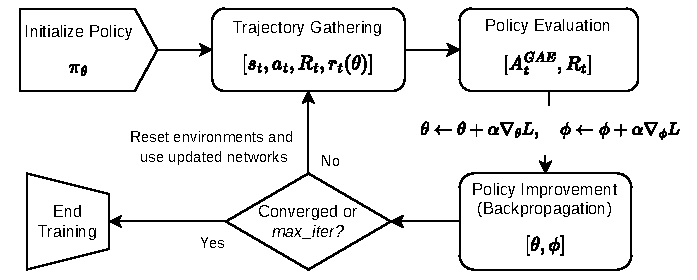
\includegraphics[width=0.8\textwidth]{diagrams/gpi.pdf}
        \caption{Generalized Policy Iteration (GPI) diagram for Policy Gradient methods.}
        \label{fig:gpi}
    \end{figure}

    Policy Gradient methods are particularly well-suited for continuous action spaces and have been widely used in finance and trading applications.
    The approach involves parameterizing the policy \( \pi_\theta(a|s) \) with a neural network and optimizing it directly to maximize the expected return.
    The policy gradient given a state-action pair \( (s, a) \) and policy network \( \pi_\theta \) is:

    \[
        \nabla_\theta J(\theta) = \mathbb{E}_{\tau \sim \pi_\theta} \left[ \sum_{t=0}^{T} \nabla_\theta \log \pi_\theta(a_t | s_t) A^\pi(s_t, a_t) \right]
    \]

    For Proximal Policy Optimization (PPO), the policy update is constrained to prevent excessive changes by using a clipped surrogate objective:

    \[
        L_{\text{actor}}(\theta) = \mathbb{E}_t \left[ \min \left( r_t(\theta) \hat{A}_t, \text{clip}(r_t(\theta), 1-\epsilon, 1+\epsilon) \hat{A}_t \right) \right]
    \]

    where \( r_t(\theta) \) is the probability ratio between the new and old policies, and \( \hat{A}_t \) is the advantage function.
    The critic loss is:

    \[
        L_{\text{critic}} = \mathbb{E}_t \left[ (V(s_t) - R_t)^2 \right]
    \]

    These updates are performed iteratively, using a neural network with backpropagation to minimize the loss and improve the policy.
    PPO ensures stability by limiting the policy update size.

    To benchmark the agent, we use a closed-form expression for the optimal bid-ask spread, as proposed by Avellaneda et al. (2008):

    \[
        \delta^* = \sigma \sqrt{2} \, \text{erf}^{-1} \left( \frac{1}{2} \left( 1 + \frac{\mu}{\sigma} \right) \right)
    \]

    where \( \sigma \) is the volatility, \( \mu \) is the mean spread, and \( \text{erf}^{-1} \) is the inverse error function.
    The optimal bid-ask spread pair is then:

    \[
        p_{\text{bid}} = \mu - \delta^*, \quad p_{\text{ask}} = \mu + \delta^*
    \]

    This closed-form expression serves as a simpler model to compare the agent's performance against a more complex environment.

    \begin{figure}[htb]
        \centering
        \includegraphics[width=0.8\textwidth]{diagrams/policy.pdf}
        \caption{Architecture of the reinforcement learning agent used in the simulation.}
        \label{fig:agent}
    \end{figure}

\end{document}